\documentclass[twocolumn,showpacs,preprintnumbers,amsmath,amssymb,floatfix,prd]{revtex4}
\usepackage{graphicx}
\usepackage{dcolumn}
\usepackage{color}
\usepackage{bm}

\newcommand*{\FigPath}{.}%  
\newcommand*{\BibPath}{.}%  
\def\AP#1{{\color{blue} #1}}


% 
\begin{document}
%
\title{Unveiling the Tensor Charge of the Nucleon at Jefferson Lab}

\author{Kalyan Allada}
\email{kalyan@jlab.org}
\affiliation{MIT}
%
\author{Jian-Ping Chen}
\email{chen@jlab.org}
\affiliation{Jefferson Lab, 12000 Jefferson Avenue, Newport News, VA 23606, USA}
%
\author{Zhong-Bo Kang}
\email{zkang@lanl.gov}
\affiliation{Theoretical Division,
                   Los Alamos National Laboratory,
                   Los Alamos, New Mexico 87545, USA}
%
\author{Nobuo~Sato}
\email{nsato@jlab.org}
\affiliation{Theory Center, Jefferson Lab, 12000 Jefferson Avenue, Newport News, VA 23606, USA}
%
\author{Alexei~Prokudin}
\email{prokudin@jlab.org}
\affiliation{Science Division, Penn State University Berks, Reading, Pennsylvania 19610, USA}
%
\author{Peng Sun}
\email{psun@msu.edu}
\affiliation{MSU}
%
\author{Zhihong Ye}\email{sassot@df.uba.ar}
\affiliation{ Physics Division, Medium Energy Group, Argonne National Lab \\
9700 S. Cass Ave, Physics Division Bldg 203, Lemont, IL 60439}
%
\author{Feng Yuan}
\email{fyuan@lbl.gov}
\affiliation{Nuclear Science Division,
                   Lawrence Berkeley National Laboratory,
                   Berkeley, California 94720, USA}



\begin{abstract}
We present detailed estimates of how well future Jefferson Lab 12 experiments, in particular CLAS and SOLID, could constrain transversity ditribution and tensor charge of the nucleon. Our study is performed based on the global QCD extraction of transversity from available experimental data and on a robust Bayesian re-weighting technique that allows to use realistic pseudo-data generated for future measurements of Jefferson Lab.
\end{abstract}

\pacs{12.38.Bx, 12.39.St, 13.85.Hd, 13.88.+e}

\maketitle

%%%%%%%%%%%%%%%%%%%%%%%%%%%%%%%%%%%%%
\section{Introduction}
%%%%%%%%%%%%%%%%%%%%%%%%%%%%%%%%%%%%%
%
Nucleon tensor charge is one of the fundamental properties
of the proton and its determination is among the main goals of
existing and future experimental facilities~\cite{Ralston:1979ys,Jaffe:1991kp,
Barone:2001sp,Dudek:2012vr,Boer:2011fh,Accardi:2012qut}.
It also plays an important role in constraining the nuclear physics aspects for
probing new physics beyond the standard model,
and has been an active subject from lattice QCD calculations~\cite{Bhattacharya:2011qm,Green:2012ej}.
In terms of the partonic structure of the nucleon, the tensor charge, $\delta q$, for a particular quark type $q$ 
is constructed from the quark transversity distribution, $h_1(x,Q^2)$,
one of the three leading-twist quark distributions that describe completely
spin-1/2 nucleon~\cite{Ralston:1979ys,Jaffe:1991kp,Barone:2001sp,Boer:2011fh}:
\begin{eqnarray}
\delta q \left(Q^2\right) \equiv   \int_{0}^{1}dx \, \left(h_1^q(x,Q^2) - h_1^{\bar q}(x,Q^2)\right)
 \ .
\end{eqnarray}


However, the experimental exploration of the quark
transversity distribution in high energy scattering is difficult
because of its odd chirality~\cite{Jaffe:1991kp}.

It is extremely important to extend the experimental study of the quark transversity
distribution to both large and small $x_B$ to constrain the total tensor charge
contributions.
The Jefferson Lab 12 GeV program~\cite{Dudek:2012vr}  is going to explore the region of relatively high-$x$ dominated by valence quarks. The planned
Electron Ion Collider~\cite{Boer:2011fh,Accardi:2012qut,Aschenauer:2014twa} is going to extend the range of explored $x$ to lower values and thus provide a possibility to study anti-quark transversity.

In this paper we will present a detailed analysis of impact of future Jefferson Lab 12 data and in particular the data from CLAS and SOLID to determination of tensor charge and transversity distributions.

We will base our studies on a QCD global fit of the available Semi-Inclusive Deep Inelastic Scattering (SIDIS) data and $e^+e^-$ annihilation into hadron pairs performed in Ref.~\cite{Kang:2015msa}. Using the best fit of transversity distributions of Ref.~\cite{Kang:2015msa} we will generate pseu-data for SOLID and CLAS experiments and estimate experimental uncertainties of future data assuming transversity distributions of Ref.~\cite{Kang:2015msa}.

The current available experimental data suggest that anti-quark transversity is very small and does not constrain anti-quark transversity. In this study we will assume that anti-quark transversity are negligible and does not contribute to tensor charge. The analysis of impact of future data including anti-quark transversity and data from future Electron-Ion Collider will be published elsewhere.

In order to analyze the impact of future data we will utilize Bayesian reweighting technique method \cite{Sato:2013ika} that will allow us to reliably estimate impact of Jefferson Lab 12 data on both quark transversity and its contribution to tensor charge.

This study will also provide information on contribution of tensor charge from kinematical region of Jefferson Lab 12 and will serve as   guidance to planning of future experiments.

%%%%%%%%%%%%%%%%%%%%%%%%%%%%%%%%%%%%%%%%%%%%%%%%%%%%%%
\section{Present status of extraction of transversity from experimental data }
%%%%%%%%%%%%%%%%%%%%%%%%%%%%%%%%%%%%%%%%%%%%%%%%%%%%%%
An important channel to investigate the quark transversity distribution is to measure the
Collins azimuthal spin asymmetries in semi-inclusive hadron
production in deep inelastic scattering (SIDIS)~\cite{Collins:1992kk}. 
Measurements have been made by the HERMES Collaboration~\cite{Airapetian:2004tw,Airapetian:2010ds}, the COMPASS Colaboration~\cite{Adolph:2012sn}, 
and JLab HALL A~\cite{Qian:2011py} experiments.
However, the extraction of the quark transversity distributions requires
the knowledge of the Collins fragmentation functions~\cite{Collins:1992kk}, which
are different from the usual unpolarized fragmentation functions. It was further
suggested to measure the Collins fragmentation functions from the 
azimuthal angular asymmetries of two back-to-back hadron productions in $e^+e^-$ annihilations~\cite{Boer:1997mf}. 
Recently both BELLE and {\em BABAR} Collaborations have studied these
asymmetries at the B-factories at center of mass energy around
$\sqrt{s}\simeq 10.6$ GeV~\cite{Abe:2005zx,Seidl:2008xc,Garzia:2012za}.
Analogous data~\cite{Ablikim:2015sma}, newly released by the BESIII collaboration, on $e^+e^-$ annihilations into pion pair at the much lower $\sqrt{s}\simeq 3.6$ GeV, offer the ideal ground for a study on the sensitivity of these azimuthal correlations on TMD evolution effects.



The data from two processes, SIDIS and $e^+e^-$, can be combined in global QCD analysis due   to the universality of the Collins fragmentation 
functions~\cite{Metz:2002iz}.
The effort to extract the transversity distributions and Collins fragmentation functions 
has been carried out by the Torino-Cagliari-JLab group extensively in the last 
few years~\cite{Anselmino:2007fs,Anselmino:2008jk,Anselmino:2013vqa,Anselmino:2015sxa}.  
Transversity coupled to the so-called dihadron interference fragmentation 
functions is employed to study transversity in its collinear version in Ref.~\cite{Radici:2015mwa}.

These results have demonstrated the powerful capability of the Collins
asymmetry measurements in constraining the quark transversity distributions 
and hence the nucleon tensor charge in high energy scattering experiments. 

The first extraction of the transversity distribution and Collins fragmentation functions with TMD 
evolution was performed in Ref.~\cite{Kang:2015msa}.
It was demonstrated  that the TMD evolution can
describe the experimental data and constrain the nucleon tensor charge with
improved theoretical accuracy.
To achieve that, the most recent developments from both theory and phenomenology 
sides~\cite{Collins:2011zzd,Yuan:2009dw,Kang:2010xv,Kang:2011mr,Echevarria:2012js,Bacchetta:2013pqa,Sun:2013hua,Echevarria:2014xaa,Echevarria:2014rua,Su:2014wpa} 
were used, and the TMD evolution at NLL order within
the Collins-Soper-Sterman (CSS)~\cite{Collins:1981uk,Collins:1984kg} formalism was applied to the data.

As our study is dedicated to Jefferson Lab 12 that will utilize SIDIS for experimental studies, let us discuss the origin of Collins asymmetries in SIDIS.

Collins asymmetries in SIDIS are generated by the convolution of the transversity function  $h_1$ and 
the Collins TMD FF $H_1^\perp$.

The relevant contributions to the SIDIS cross-sections are
\begin{align}
\frac{d^5\sigma(S_\perp)}{dx_B dy dz_h d^2P_{h\perp}}
= \sigma_0(x_B, y, Q^2)
\Big[F_{UU} +   \nonumber \\ 
  \sin(\phi_h+\phi_s)\,
\frac{2 (1-y)}{1+(1-y)^2} \, F_{UT}^{\sin\left(\phi_h +\phi_s\right)} + ... \Big]\,.
  \label{eq:aut-collins}
\end{align}
%
The polarized structure function $F_{UT}^{\sin\left(\phi_h +\phi_s\right)}$ contains the convolution of transversity 
with the Collins function, $h_1 \otimes H_1^\perp$.

Experimentally measured Collins asymmetry is then
\begin{align}
A_{UT}^{\sin\left(\phi_h +\phi_s\right)}(x_B, y, z_h, P_{h\perp})
=  
\frac{2 (1-y)}{1+(1-y)^2} \, \frac{F_{UT}^{\sin\left(\phi_h +\phi_s\right)}}{F_{UU}}  
  \label{eq:aut-collins1}
\end{align}


Applying the TMD evolution, $F_{UU}$ and $F_{UT}^{\sin\left(\phi_h +\phi_s\right)}$ can be written as~\cite{Collins:1981uk,Collins:1984kg,Boer:2001he,Kang:2011mr}
\begin{eqnarray}
F_{UU} &=& \frac{1}{z_h^2}\int \frac{db\, b}{2\pi} J_0\!\!\left( \frac{{P}_{h\perp} b}{z_h} \right)\,
e^{-S_{\rm PT}(Q,b_*)-S_{\rm NP}^{\rm (SIDIS)}(Q,b)}  \nonumber\\
&\times & \, C_{q\leftarrow i}\otimes f_{1}^{i}(x_B,\mu_b)  \,\,\,
\hat{C}_{j\leftarrow q}^{\rm (SIDIS)}\otimes \hat D_{h/j}(z_h,\mu_b), \nonumber \\ ~ \label{fuu}\\
F_{UT}^{\sin\left(\phi_h +\phi_s\right)} &=& -\frac{1}{2 z_h^3} \int \frac{db \, b^2}{2\pi} J_1\!\!\left( \frac{{P}_{h\perp} b}{z_h} \right)\,
e^{-S_{\rm PT}(Q,b_*)-S_{\rm NP\, coll}^{\rm (SIDIS)}(Q,b)} \nonumber\\
&\times & \, \delta C_{q\leftarrow i}\otimes h_{1}^{i}(x_B,\mu_b)  \,\,\,
\delta \hat{C}_{j\leftarrow q}^{\rm (SIDIS)}\otimes \hat H_{h/j}^{(3)}(z_h,\mu_b) , \nonumber \\ 
~\label{eq:fut1}
\end{eqnarray}
%
where $b$ is the Fourier conjugate variable to the measured final hadron
momentum ${P}_{h\perp}$, $J_1$ is
the Bessel function, $\mu_b=c_0/b_*$ with $c_0\simeq 1.12$, and the symbol
$\otimes$ represents the usual convolution in momentum fractions.
The sum over quark flavors $q$ weighted with quark
charge, $\sum_q e^2_q$, and the sum over $i,j = q,\bar q, g$, are 
implicit in all formulas for the structure functions. 
$C$, $\hat{C} $ and $\delta C$, $\delta \hat{C} $ are the coefficient functions for the unpolarized distribution and fragmentation functions, 
and for transversity and Collins FF, that can be calculated perturbatively.
% 
%%%%%%%%%%%%%%%%%%%%%%%%%%%%%%%%%%%%%%%%%%%%%%%%%%%%%%%
 \begin{figure}
 \centering
% \vspace*{0.9cm}
 \resizebox{0.38\textwidth}{!}{ 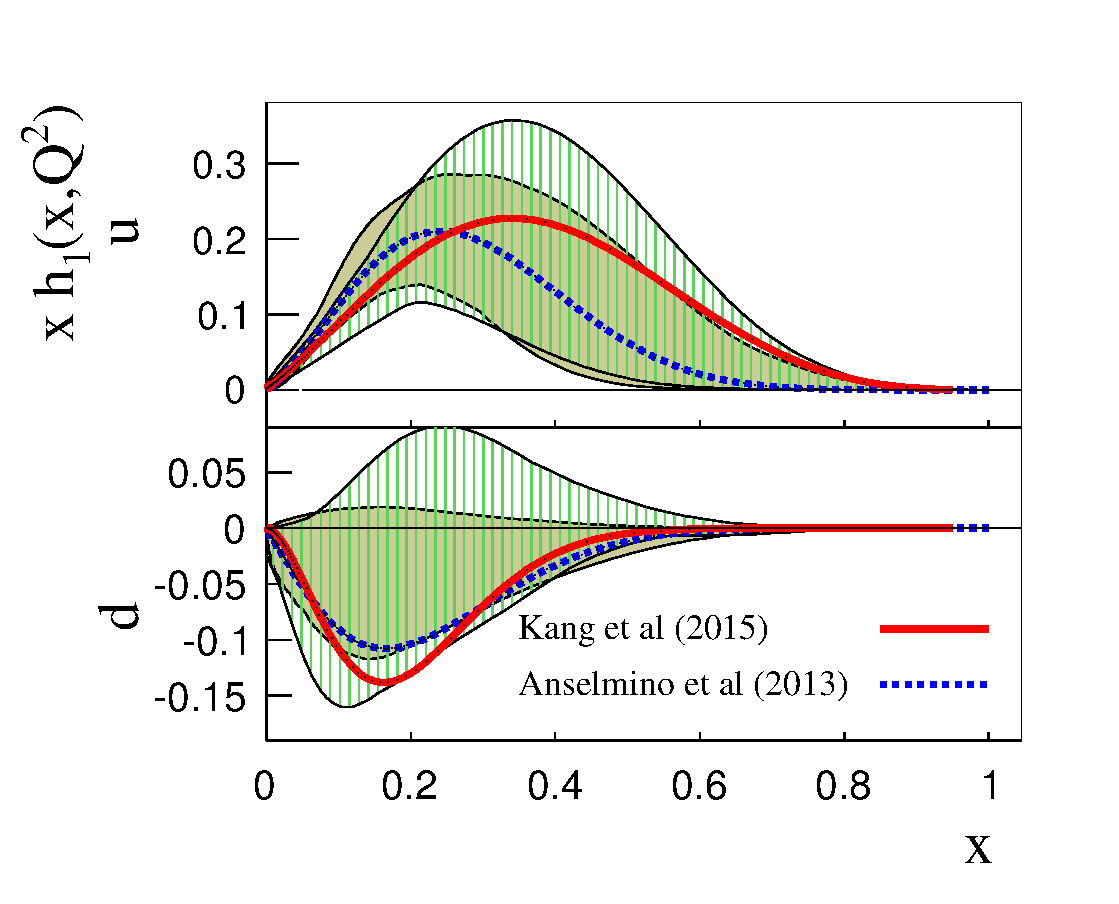
\includegraphics{\FigPath/transversity_comparison.pdf} }\\
  \caption{[color online] Transversity distribution for up and down quarks comparison of extraction in 
 Ref.~\cite{Kang:2015msa} and \cite{Anselmino:2013vqa}. The band corresponds to the uncertainty of 
 the extraction. 
  }
 \label{fig:transversity}
 \end{figure}
%%%%%%%%%%%%%%%%%%%%%%%%%%%%%%%%%%%%%%%%%%%%%%%%%%%%%%%%
%
The usual $b_*$-prescription that allows for smooth transition from perturbative to non perturbative physics was used in Ref.~\cite{Kang:2015msa}. $S_{\rm NP}^{\rm (SIDIS)}$ and $S_{\rm NP\, coll}^{\rm (SIDIS)}$ are non perturbative factors contain information on the initial conditions of evolution:
\begin{align}
S_{\rm NP}^{\rm (SIDIS)} &= g_2 \ln\left(\frac{b}{b_*}\right)\ln\left(\frac{Q}{Q_0}\right)+\left({g_q}+\frac{g_h}{z_h^2}\right)b^2 \ , \\
S_{\rm NP\, collins}^{\rm SIDIS} &=g_2 \ln\left(\frac{b}{b_*}\right)\ln\left(\frac{Q}{Q_0}\right)+\left({g_q}+\frac{g_h-g_c}{z_h^2}\right)b^2 \ ,
\label{eq:sud_np}
\end{align}
where  $Q_0^2$ = 2.4 GeV$^2$, for the spin-averaged   contribution.
In the above parameterization, the parameters $g_q = g_1/2=0.106$, $g_2=0.84$, $g_h=0.042$  (GeV$^2$) have been determined
from the analysis of SIDIS and Drell-Yan processes in Ref.~\cite{Su:2014wpa}.  

The existing experimental data does not allow to determine precisely shapes of all polarised distributions in
 coordinate space,  the parameter $g_c$ allowed for the Collins fragmentation function to modify
 its shape with respect to unpolarised fragmentation distributions. 


The Collins fragmentation function $H_{1\, h/j}^\perp(z_h,p_\perp)$ ~\cite{Collins:1992kk} at small values of $b$ can be reated to the so called twist-three fragmentation function $\hat{H}_{h/q}^{(3)}(z_h)$ ~\cite{Yuan:2009dw} via Operator Product Expansion (OPE).

Three important ingredients have to be included to achieve the NLL
formalism for the above structure functions and asymmetries.
First of all, the perturbative Sudakov form factor~\cite{Koike:2006fn},
\begin{equation}
S_{\rm PT}(Q,b_*)=\int_{\mu_b^2}^{Q^2}\frac{d\mu^2}{\mu^2}\left[A\ln\frac{Q^2}{\mu^2}+B\right] \ ,\label{eq:spert}
\end{equation}
with perturbative coefficients $A^{(1,2)}\sim{\alpha_s^{(1,2)}}$ and $B^{(1)}\sim{\alpha_s^1}$~\cite{Nadolsky:1999kb,Koike:2006fn}.
Then, the scale evolutions of the quark trans\-ver\-si\-ty distribution and of the Collins fragmentation functions up to the scale of $\mu_b$.


The global fit of SIDIS and $e^+e^-$ was performed in Ref.~\cite{Kang:2015msa}. 
The quark transversity distributions was parametrized as
as
\begin{align}
h_1^{q}(x,Q_0)= & N_{q}^h x^{a_{q}}(1-x)^{b_{q}} \frac{(a_{q} + b_{q})^{a_{q} + b_{q}}}
{a_{q}^{a_{q}} b_{q}^{b_{q}}}\nonumber \\
\times & \frac{1}{2}\left (f_{1}^q(x,Q_0) + g_{1}^q(x,Q_0)  \right ) \ ,
\end{align}
at the initial scale $Q_0$, for up and down quarks $q=u,d$, respectively, where $f_{1}^q$ are the unpolarized
CT10 NLO quark distributions~\cite{Lai:2010vv} and $g_{1}^q$ are the NLO DSSV quark helicity distributions~\cite{deFlorian:2009vb}. The available SIDIS data does not allow for extraction of anti-quark transversity distributions and anti-quark transversity was assumed to be zero, $h_1^{\bar q} = 0$. 

Twist-3 Collins fragmentation functions were parametrized in terms of the unpolarized fragmentation functions,
\begin{align}
\hat{H}_{fav}^{(3)}(z,Q_0)&= N_{u}^c z^{\alpha_{u}}(1-z)^{\beta_{u}} D_{\pi^+/u}(z,Q_0) \ , \\
\hat{H}_{unf}^{(3)}(z,Q_0)&= N_{d}^c z^{\alpha_{d}}(1-z)^{\beta_{d}} D_{\pi^+/d}(z,Q_0) \ , 
\end{align}
which correspond to the favored and unfavored Collins
fragmentation functions, respectively. 
  The newest NLO extraction of fragmentation functions~\cite{deFlorian:2014xna} was used for unpolarised FF, $D$. 
  
  
 
 
 Therefore, Ref.~\cite{Kang:2015msa} introduced total of 13 parameters in the global fit:
 $N_u^h$, $N_d^h$, $a_u$, $a_d$, $b_u$, $b_d$, $N_u^c$, $N_d^c$, $\alpha_u$, $\alpha_d$, $\beta_d$, $\beta_u$, $g_c$ (GeV$^2$).  

 The global fit of SIDIS and $e^+e^-$ data  resulted in the total  $\chi^2 =  218.407 $, $n_{d.o.f.} = 249$, and 
$\chi^2/n_{d.o.f} = 0.88$. The description of the data was  equally good for SIDIS and $e^+e^-$:  $\chi^2_{SIDIS}/{n_{SIDIS}} =  0.93$, $\chi^2_{e^+e^-}/{n_{e^+e^-}} =  0.72$.  

The resulting parameters of  Ref.~\cite{Kang:2015msa} after minimization procedure are presented in Table~\ref{parameters}.

\begin{table}[htb]
\begin{tabular}{l c l l c l l c l}
\hline
 & & & & & & & &\\
$N_u^h$ &=& $0.85\pm 0.09$ & $a_u$ &=& $ 0.69 \pm 0.04$ & $b_u$ &=& $ 0.05 \pm 0.04$ \\
$N_d^h$ &=& $-1.0\pm 0.13$ & $a_d$ &=& $ 1.79 \pm 0.32$ & $b_d$ &=& $ 7.00 \pm 2.65$  \\
$N_u^c$ &=& $-0.262\pm 0.025$ & $\alpha_u$ &=& $ 1.69 \pm 0.01$ & $\beta_u$ &=& $ 0.00 \pm 0.54$ \\
$N_d^c$ &=& $0.195\pm 0.007$ & $\alpha_d$ &=& $ 0.32 \pm 0.04$ & $\beta_d$ &=& $ 0.00 \pm 0.79$ \\
$g_c$ &=& $0.0236\pm 0.0007$&\multicolumn{3}{l}{(GeV$^2$)}\\
& & & & & & & &\\
\hline
& & & & & & & &\\
\multicolumn{3}{l}{$\chi_{min}^2 =  218.407$} & \multicolumn{3}{l}{$\chi^2_{min}/{n.d.o.f}=0.88$}  \\
\end{tabular}
\caption{Fitted parameters of the transversity quark distributions for $u$ and $d$ and Collins fragmentation functions.}
\label{parameters}
\end{table}

Fig.~\ref{fig:transversity}  shows transversity distributions for $u$ and $d$ quarks results obtained in Ref.~\cite{Kang:2015msa} and compared to results of   Ref.~\cite{Anselmino:2013vqa}. 


Since the experimental data has only probed the limited region $0.0065 < x_B < 0.35$,
 the following partial contribution to the tensor charge was defined
\begin{eqnarray}
\delta q^{[x_{\rm min},x_{\rm max}]}\left(Q^2\right) \equiv   \int_{x_{\rm min}}^{x_{\rm max}}dx \, h_1^q(x,Q^2) \ .
\end{eqnarray}
and the following partial tensor charges were calculated ~\cite{Kang:2014zza}
\begin{eqnarray}
\delta u^{[0.0065,0.35]} &=&  +0.30_{-0.12}^{+0.08} \ ,\\
\delta d^{[0.0065,0.35]} &=&  -0.20_{-0.11}^{+0.28}   \ ,
\end{eqnarray}
at 90\% C.L. at  $Q^2=10$ GeV$^2$.

The tensor charge calculated over the whole kinematical region $\delta q^{[0,1]}$ is:
\begin{eqnarray}
\delta u^{[0,1]} &=&  +0.39_{-0.20}^{+0.16} \ ,\\
\delta d^{[0,1]} &=& -0.22_{-0.10}^{+0.31} \ ,
\end{eqnarray}
at 90\% C.L.

One can see that the kinematical region not covered by experimental data can potentially give $\sim 25$\% contribution to the tensor charge.

Apart from that the assumption that anti-quark transversity is exactly equal to zer may not be true in future and maximal contribution from see quarks can be ....
for $\bar u$ and $\bar d$ quarks respectively.


The isoscalar nucleon tensor charge $g_T^0= \delta u + \delta d$ is
\begin{eqnarray}
g_T^0 = +0.17^{+0.47}_{-0.30} \, ,
\end{eqnarray}
at 90\% C.L. at  $Q^2=10$ GeV$^2$.



%%%%%%%%%%% FIG %%%%%%%%%%%
\begin{figure}[tbp]
\centering
 \resizebox{0.38\textwidth}{!}{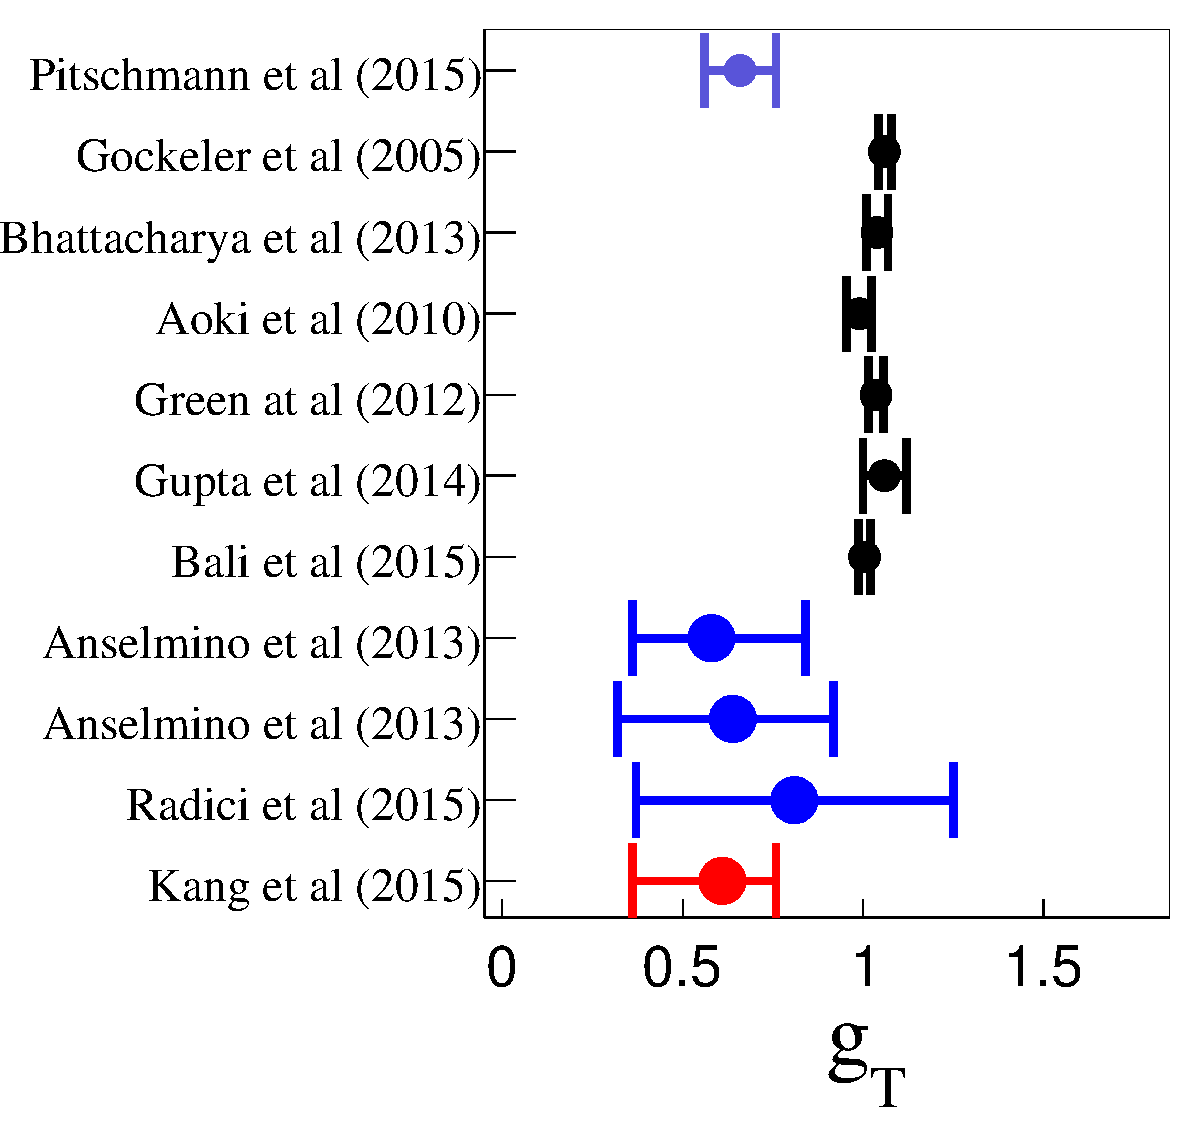
\includegraphics{\FigPath/gt_comparison.pdf} }\\
\caption{[color online] Comparison of the isovector nucleon tensor charge $g_T$   from this paper at 68\% C.L. (Kang et al 2015) at $Q^2=10$ GeV$^2$ and result from Ref.~\cite{Radici:2015mwa}  (Radici et al 2015) at 68\% CL and  $Q^2=4$ GeV$^2$,
and Ref.~\cite{Anselmino:2013vqa} at 95\% CL standard and polynomial fit (Anselmino et al 2013) at $Q^2=0.8$ GeV$^2$. Other points are lattice computation  at $Q^2=4$ GeV$^2$ of Bali et al Ref.~\cite{Bali:2014nma},  Gupta et al Ref.~\cite{Gupta:2015tpa}, Green et al Ref.~\cite{Green:2012ej}, Aoki et al Ref.~\cite{Aoki:2010xg}, Bhattacharya et al  ref.~\cite{Bhattacharya:2013ehc}, Gockeler et al Ref.~\cite{Gockeler:2005cj}. Pitschmann et al is DSE calculation at $Q^2=4$ GeV$^2$  Ref.~\cite{Pitschmann:2014jxa}.}
\label{fig:comparison_gt}
\end{figure}
%%%%%%%%%%% FIG %%%%%%%%%%%
  
The isoscalar tensor charge is presented in Fig.~\ref{fig:comparison_gt}. 
One can see that lattice QCD calculations have much better precision compared to extractions from experimental data.

Future Jefferson Lab 12 data is going to allow for much more precise extraction of tensor charge that will compete with ab-initio calculations.

%%%%%%%%%%%%%%%%%%%%%%%%%%%%%%%%%%%%%%%%%%%%%%%%%%%%%%%%%%%%%%%%%
\section{Bayesian re-weighting technique}
%%%%%%%%%%%%%%%%%%%%%%%%%%%%%%%%%%%%%%%%%%%%%%%%%%%%%%%%%%%%%%%%%
%
\AP{Nobuo, could you write description of the re-weighting procedure, please?}
Bayes theorem allows to incorporate information from new data by applying re-weighting of probability densities for model parameters. The details of application of re-weighting are explained in Ref.~\cite{Sato:2013ika}.

Probability density function for model parameters $\bm{\alpha}$, $\mathcal{P}(\bm{\alpha})$, is going to be modified in presence of new data and the Bayes theorem states that 
%
\begin{align}
\mathcal{P}(\bm{\alpha}|D)
=\frac{\mathcal{P}(D|\bm{\alpha})}{\mathcal{P}(D)} \mathcal{P}(\bm{\alpha}),
\label{eq:bayes}
\end{align}
%
where $\mathcal{P}(\bm{\alpha}|D)$ is the so-called \emph{posterior} density, 
is the updated pdf from the \emph{prior} density 
$\mathcal{P}(\bm{\alpha})$.
 
The quantity $\mathcal{P}(D|\bm{\alpha})$ called the \emph{likelihood} 
function,
represents the conditional probability for a data set $D$ given the
parameters $\bm{\alpha}$ of the model.
The quantity $\mathcal{P}(D) $ ensures the normalization of the 
posterior density to unity.  

For a particular observable $\mathcal{O}$ one can write the expectation value 
with the new data as,
%
\begin{align}
\text{E}[\mathcal{O}]
&=	\int d^n\alpha \mathcal{P}(\bm{\alpha}|D)
	\mathcal{O}(\bm{\alpha})\notag\\
&=	\int d^n\alpha \frac{\mathcal{P}(D|\bm{\alpha})}{\mathcal{P}(D)} 
	\mathcal{P}(\bm{\alpha})\mathcal{O}(\bm{\alpha})\notag\\
&=	\frac{1}{N} \sum_k w_k \mathcal{O}(\bm{\alpha}_k).
\label{eq:E}
\end{align}
%
In the last line  a Monte Carlo approximation of the integral is used.
Similarly, the variance is of observable $\mathcal{O}$ is given by
%
\begin{align}
\text{Var}[\mathcal{O}]
&=\frac{1}{N} \sum_k w_k (\mathcal{O}(\bm{\alpha}_k)-\text{E}
[\mathcal{O}])^2 .
\label{eq:Var}
\end{align}
%
The quantities $\{w_k\}$ are called \emph{weights} and are proportional to 
$\mathcal{P}(D|\bm{\alpha}_k)$. 
Their normalization is fixed by demanding $\text{E}[1]=1$, that is,  
$\sum_k w_k=N$.
%----------------------% 

The reweighting procedure depends on the form assumed for the likelihood 
function. We use $\chi^2$ minimization in the fits and thus weights have the following form:
\begin{align}
	w_k \propto \exp\left(-\frac{1}{2}\chi^2\right),
\label{eq:bayes1}
\end{align}



%%%%%%%%%%%%%%%%%%%%%%%%%%%%%%%%%%%%%%%%%%%%%%%%%%%%%%%%%%%%%%%%%%%%%%%%%%%%%%
\section{Simulated Data for Jefferson Lab}
%%%%%%%%%%%%%%%%%%%%%%%%%%%%%%%%%%%%%%%%%%%%%%%%%%%%%%%%%%%%%%%%%%%%%%%%%%%%%%
%
\AP{Zhihong, Kalyan, could you write description of CLAS, SOLID and how data were generated, please?}
 
%
%%%%%%%%%%%%%%%%%
%%%TABLE I
%%%%%%%%%%%%%%%%
%
\begin{table}[bth!]
\begin{tabular}{ccccc}
\end{tabular}
\caption{\label{tab:kinem} Pseudo-data generated and kinematical limits of SOLID.}
\end{table}
%


%%%%%%%%%%%%%%%%%%%%
% FIGURE 1
%%%%%%%%%%%%%%%%%%%
%
\begin{figure}[thb!]
\vspace*{-0.4cm}
\begin{center}
\vspace*{-0.6cm}
 \end{center}
\vspace*{-0.7cm}
\caption{\label{fig:kimen} [color online]
Kinematical plane with Jefferson Lab data.}
\end{figure}
%
 

%%%%%%%%%%%%%%%%%%%%%%%%%%%%%%%%%%%%%%%%%%%%%%%%%%%%%%%%%%%%%%%%%%%%%%%%%%%%%%
\section{Tensor charge and transversity from CLAS}
%%%%%%%%%%%%%%%%%%%%%%%%%%%%%%%%%%%%%%%%%%%%%%%%%%%%%%%%%%%%%%%%%%%%%%%%%%%%%%
 
%%%%%%%%%%%%%%%%%%%%%%%%%%%%%%%%%%%%%%%%%%%%%%%%%%%%%%%%%%%%%%%%%%%%%%%%%%%%%%
\section{Tensor charge and transversity from SOLID}
%%%%%%%%%%%%%%%%%%%%%%%%%%%%%%%%%%%%%%%%%%%%%%%%%%%%%%%%%%%%%%%%%%%%%%%%%%%%%%

%%%%%%%%%%%%%%%%%%%%%%%%%%%%%%%%%%%%%%%%%%%%%%%%%%%%%%
\section{Summary and Conclusions}
%%%%%%%%%%%%%%%%%%%%%%%%%%%%%%%%%%%%%%%%%%%%%%%%%%%%%%
%
 

%%%%%%%%%%%%%%%%%%%%%%%%%%%
\section*{Acknowledgments}
%%%%%%%%%%%%%%%%%%%%%%%%%%%
%
We are grateful to  
This work was partially supported by   the
U.S.\ Department of Energy under Contract No.~ .

%%%%%%%%%%%%%%
\bibliography{\BibPath/solid}
 
\end{document}














